Un análisis claro y un diseño conciso no garantizan que, a la hora de
implementar el sistema planteado, no se encuentre ninguna dificultad o
imprevisto. Así pues, en este capítulo comentaremos los retos y detalles que más
relevancia o complejidad han presentado durante la fase de la implementación del
proyecto.

De igual modo, durante el desarrollo de la aplicación se mantuvo actualizada una
bitácora, accesible en línea~\cite{ofluteblog}, en la que se fueron detallando,
a medida que aparecían, muchas de estas dificultades.

Como complemento a la lectura de este capítulo se recomienda tener una copia
local del repositorio del proyecto, disponible para su libre descarga desde la
forja oficial~\cite{ofluteforja}. En él se encuentra todo el código fuente
original, así como la documentación en formato \textit{Doxygen}~\cite{doxygen}.

\section{Carga y uso de fuentes TrueType en Gosu}

Como se ha comentado previamente, \textbf{oFlute} hace uso de la biblioteca
\textit{Gosu}, que proporciona una API sencilla para el acceso al sistema
gráfico, entre otras características. Este framework funciona en sistemas
Windows, GNU/Linux y Mac OS, aunque dada la dificultad de conseguir la
compatibilidad con todos ellos, la calidad y el rendimiento es bastante
desigual de un sistema a otro.

Una de estas desigualdades se presentaba a la hora de \textbf{cargar fuentes}
para mostrar textos. En su versión para GNU/Linux, el módulo para el pintado de
textos de Gosu (que comprende la clase \texttt{Gosu::Font} y las funciones
\texttt{Gosu::drawText} y \texttt{Gosu::createText}) solo permitía
utilizar fuentes que estuvieran ya instaladas en el sistema de forma global, de
modo que era imposible adjuntar un fichero con una fuente en formato
\texttt{TrueType}~\cite{reftruetype} para su carga en el juego. 

La instalación de fuentes en sistemas GNU/Linux siempre ha sido una operación
engorrosa que ha requerido permisos de administrador. Esto, unido a que tanto en
Windows como en Mac OS la opción de cargar fuentes desde un fichero sí estaba
disponible, supuso un grave problema en el planteamiento del proyecto.

Inicialmente se investigaron las razones de esta limitación. Al ser un proyecto
libre y abierto, revisamos el código de Gosu, concretamente la implementación
de la clase \texttt{Gosu::Font} previamente citada, de la que dependían todas
las otras funciones relacionadas con fuentes.

Las conclusiones que se sacaron fueron que Gosu, bajo GNU/Linux, implementaba el
renderizado de fuentes mediante una biblioteca llamada Pango~\cite{Pango}, de
bastante bajo nivel, y que por diseño está limitada al uso de fuentes de
sistema, ya que se orienta a herramientas del sistema operativo, no a
aplicativos de terceros.

Así pues, era necesario buscar una alternativa. En numerosos proyectos
previos~\cite{robinson} se había utilizado la biblioteca
\textbf{SDL}~\cite{refsdl}, un framework multimedia muy utilizado en
aplicaciones de audio, vídeo y juegos. Uno de los subsistemas que proporciona
SDL es \textbf{SDL\_ttf}~\cite{refsdlttf}, una biblioteca para el renderizado de
fuentes basadas en ficheros \texttt{TrueType}. Esto, unido a que la propia SDL
ya era una dependencia de Gosu, propició que se iniciara la implementación de
una solución basada en este medio.

\subsection{Funcionamiento de \texttt{SDL\_ttf}}

Para comprender cómo se implementó la solución al problema citado, el primer
paso es entender cómo funciona la biblioteca \texttt{SDL\_ttf} para poder ver
cómo se corresponde luego con Gosu.

\subsubsection{Tipos de datos utilizados}

En común con el resto de módulos de SDL, SDL\_ttf se basa en un tipo de datos
conocido como \textit{superficies} (\texttt{SDL\_Surface}). Estas superficies
representan mapas de bits cargados en memoria, y se utilizan para guardar las
imágenes que se cargan de los ficheros, así como para representar otros destinos
gráficos intermedios, como la propia pantalla.

Para representar el color del texto que vamos a pintar, SDL\_ttf utiliza la
estructura \texttt{SDL\_Color}, que guardará los valores de color de 8 bits para
los tres canales de color primario (rojo, verde y azul).

Además, SDL\_ttf define un tipo de datos propio, de nombre \texttt{TTF\_Font}, que
representa una fuente cargada a partir de un fichero, con un tamaño determinado.

\subsubsection{Funciones utilizadas}

SDL\_ttf precisa de una \textbf{inicialización} previa, que se lleva a cabo mediante la
llamada a \texttt{TTF\_Init()}. Igualmente, liberaremos los recursos ocupados
mediante \texttt{TTF\_Quit()}.

Para \textbf{cargar la fuente} a partir de los ficheros TrueType (con extensión
\texttt{.ttf}), se utiliza la función \texttt{TTF\_OpenFont(const char * fichero,
  int tamaño)}. Esta función recibe una cadena con el nombre del fichero y el
tamaño de letra a utilizar, y devuelve un puntero al tipo \texttt{TTF\_Font}.

\begin{minted}{cpp}
  TTF_Font * fuente = TTF_OpenFont("fichero_fuente.ttf", 25);
\end{minted}

Una vez cargada la fuente de nuestro interés, tendremos que \textbf{generar una
  superficie} con el texto que queramos. Para ello, SDL\_ttf ofrece una gran
variedad de funciones, según el suavizado del texto y el tipo de caracteres que
estemos utilizando. En nuestro caso, queríamos que la superficie tuviera fondo
transparente, así como usar caracteres en UTF-8~\cite{refutf8}, por lo que la
función que se eligió fue 
\begin{minted}{cpp}
  SDL_Surface * TTF_RenderUTF8_Blended (TTF_Font * fuente,
                                        const char * texto,
                                        SDL_Color color);
\end{minted}

Esta función devolverá un puntero a una superficie que se integrará
(\textit{blends}) sobre cualquier imagen, al tener el fondo transparente.


\subsection{Representación de imágenes en Gosu}

Una vez conocidos los tipos de datos y funciones que ofrece SDL\_ttf, es
necesario conocer cuáles son los tipos de datos equivalentes en Gosu, de forma
que pueda haber una \textit{conversión} de un tipo a otro.

\subsubsection{Mapas de bits de bajo nivel: Gosu::Bitmap}
La clase \texttt{Gosu::Bitmap} representa, en Gosu, un mapa de bits de bajo
nivel. Éste no contará con aceleración por hardware ni podrá mostrarse en
pantalla, pero podremos acceder directamente a los datos de los píxeles y
trabajar con ellos.

\texttt{Gosu::Bitmap} nos servirá de paso intermedio entre la superficie de SDL y las
imágenes habituales de Gosu.

\subsubsection{Imágenes de uso común: Gosu::Image}
En Gosu las imágenes y assets gráficos se manejan habitualmente con la clase
\texttt{Gosu::Image}, que representa un contenedor de más alto nivel que
\texttt{Gosu::Bitmap}, además de estar optimizado y poder pintarse en pantalla.

Podremos crear un objeto de esta clase a partir de un \texttt{Gosu::Bitmap}, consiguiendo
finalmente un objeto \textit{pintable}.


\subsection{Implementación final}

Conocidas las representaciones internas de ambas bibliotecas, la implementación
final fue una clase con una interfaz similar a \texttt{Gosu::Font}, de modo que
la transición pudiera ser lo más transparente posible, de nombre
\texttt{CustomFont}.

En el constructor se inicializa (de forma única, mediante una variable estática)
el subsistema \texttt{SDL\_ttf} utilizando la llamada
\texttt{TTF\_Init()}. Después, se carga la fuente indicada por los parámetros
del constructor. En ambos casos, se comprueba que el procedimiento ha sido
correcto, lanzando una excepción en caso contrario.

\begin{minted}{cpp}
static int initResult = TTF_Init();
if (initResult < 0)
   throw std::runtime_error("Could not initialize SDL_TTF");

font = TTF_OpenFont(fontName, fontHeight);
if (!font)
   throw std::runtime_error("Could not open TTF file " + fontName);

\end{minted}

Seguidamente, en el método de pintado (\texttt{draw}) se genera la superficie
con el texto que se indique, pasando el contenido de los píxeles a un contenedor
\texttt{Gosu::Bitmap} y finalmente generando un objeto \texttt{Gosu::Image} a
partir del mismo.

\begin{minted}{cpp}
SDL_Surface * surf = TTF_RenderUTF8_Blended(font, text, color);
if (!surface)
   throw std::runtime_error("Could not generate the surface");

Gosu::Bitmap temp;
temp.resize(surf.width(), surf.height());
std::memcpy(temp.data(), surf.data(), temp.width() * temp.height() * 4);

Gosu::Image image (graphic_target, temp);
image.draw(x, y, z);
\end{minted}

\subsection{Recepción}

Una vez contamos con una implementación funcional de la clase, se presentó el
parche en el foro oficial de Gosu~\cite{foroGosu}. En poco tiempo, el
desarrollador principal verificó el código propuesto e hizo una adaptación al
propio código original de la clase \texttt{Gosu::Font} para añadir la
propuesta. 

Por ende, desde la versión 0.7.20, el \textit{parche} forma parte
oficial de Gosu, y así se hace indicar en el fichero \texttt{TextUnix.cpp} de la
distribución oficial:

\begin{minted}{cpp}
// [...]

// Used for custom TTF files
// Adapted from customFont class by Jose Tomas Tocino Garcia (TheOm3ga)
class SDLTTFRenderer : boost::noncopyable

// [...]
\end{minted}

Así pues, dado que la solución propuesta se integró en la distribución oficial,
nos deshicimos de la clase \texttt{customFont} a favor de la actualización de
\texttt{Gosu::Font}, dado que al fin y al cabo el funcionamiento interno es
el mismo.

\section{Animaciones dinámicas}
\label{sec:animaciones}

Una de las decisiones iniciales de diseño fue la de hacer la interfaz gráfica de
usuario lo más atractiva posible, intentando utilizar gráficos amigables y, en
la medida de lo posible, animaciones y efectos dinámicos.

Con esto, se tornaba necesario crear un sistema de animaciones lo más versátil
posible, de forma que dotar a los elementos de la interfaz de movimiento fuera
un proceso sencillo. 

\subsection{Antecedentes: animaciones en Flash}
Para evitar reinventar la rueda y tener una base estable con la que empezar, se
investigaron sistemas de animaciones ya existentes, evaluando diferentes
enfoques y aproximaciones, sobre todo en sistemas altamente relacionados con las
animaciones. En particular, nos centramos en Adobe Flash (\textit{anteriormente
  Macromedia Flash}) y la gran cantidad de código disponible relacionado con la
generación de animaciones dinámicas.

Especialmente interesante es el trabajo de Robert Penner, un programador
americano muy interesado en la programación matemática, que ideó un sistema de
animaciones dinámicas para ActionScript~\cite{actionscript} 1.0 y 2.0. Penner,
en su libro \textit{Programming Macromedia Flash MX}~\cite{libropenner} incluyó
un capítulo llamado \textit{Motion, Tweening and Easing} (que dada su
popularidad acabó ofreciendo de forma gratuita~\cite{capitulopenner}), en el que
por primera vez presentó y explicó con detalle su sistema de animaciones.

En el citado capítulo se desgranan las animaciones como ecuaciones dependientes
del tiempo y de las posiciones inicial y final, de forma que fuera fácil generar
una serie de funciones para determinar la posición de un objeto en cada
instante. Una vez presentados los conceptos iniciales, Penner desvela una serie
de ecuaciones de movimiento (que acabaron siendo bautizadas y mundialmente
conocidas como las \textit{Penner's Easing Equations}). Estas ecuaciones modelan
un gran número de movimientos, en función de cómo varía la posición respecto del
tiempo (y perceptualmente la aceleración/deceleración del objeto animado).

Además, por cada tipo de ecuación, Robert Penner generó tres tipos de
movimientos: de aceleración (\textit{ease in}), de deceleración o frenada
(\textit{ease out}), y de aceleración-deceleración (\textit{ease in-out}). Con
esto, quedaban cubiertas la práctica totalidad de los tipos de animaciones posibles.

Así, un ejemplo de ecuación podrían ser las cúbicas, que hacen que la posición
del movimiento se rija por una función cúbica del tiempo. Si graficamos la
relación del tiempo por la posición, ambos de 0 a 1, el resultado sería el
siguiente:

\begin{gnuplot}
set xrange [0:1]
set yrange [0:1]
set size square
set nokey
set xlabel "tiempo"
set ylabel "posición"
plot x*x*x
\end{gnuplot}

Tras estudiar bien el código original, se decidió hacer una adaptación en C++,
de forma que se adaptara a las necesidades del proyecto.

\subsection{Adaptación en C++}
El primer paso fue portar las ecuaciones propiamente dichas -- esto es, las
funciones que generaban las posiciones intermedias. Dado que el lenguaje
original, ActionScript, es un derivado de EcmaScript~\cite{Ecmascript}, la
sintaxis es prácticamente idéntica a C++ en cuanto a asignaciones y operadores
se refiere, por lo que este paso fue prácticamente transparente.

Seguidamente, se ideó un \textit{wrapper} para estas ecuaciones, de forma que
fuera un objeto independiente el que se encargara de calcular las posiciones
intermedias de la animación, en lugar de tener que hacerlo los propios objetos
animados. Para ello, se creó la clase \texttt{Animación}, con las siguientes
características:
\begin{itemize}
\item Para cada instancia, permite animar un número arbitrario de valores, de
  forma que con un solo objeto \textit{Animacion} podamos animar la posición
  horizontal y vertical de un objeto, por ejemplo.
\item Permite elegir entre tres tipos de movimiento (\textit{ease in},
  \textit{ease out} y \textit{ease in-out}) para tres ecuaciones distintas
  (cuadrática, cúbica y cuártica), además de una ecuación especial con
  movimiento de ida y vuelta, y, lógicamente, movimiento uniforme. En total, 11
  posibles movimientos.
\item Capacidad para atrasar las animaciones, de forma que sea sencillo generar
  animaciones escalonadas de varios elementos sin tener que recurrir a
  \textit{callbacks}.
\end{itemize}

\subsection{Ejemplo de uso}

Supongamos que tenemos una pelota que queremos mover diagonalmente con un
movimiento de aceleración, desde la posición 0,0 hasta la posición 150, 300, en
30 pasos. Además, tenemos un cuadrado que habrá de moverse de la posición 0, 150
hasta la posición 150,150 cuando la pelota vaya por la mitad de su camino, y que
llegue a la vez que aquella.

Para cumplir este objetivo, crearemos dos objetos \texttt{Animación}, uno para
la pelota y otro para el cuadrado. En el caso de la pelota estaremos animando
dos parámetros, la posición horizontal y la vertical, y la duración será de 30
pasos. El tipo de movimiento será de aceleración, y la ecuación que elegiremos
será la cuadrática. Al no indicarse nada, no habrá espera inicial.

\begin{minted}{cpp}
// Creamos la instancia
Animacion animPelota (2, 30, Animacion::tEaseInQuad, 0);

// Asignamos la pos inicial y final de la coordenada horizontal
animPelota.set(0, 0, 150);  

// Coordenada vertical
animPelota.set(1, 0, 300);
\end{minted}

En el caso del cuadrado el movimiento sólo será horizontal, por lo que
animaremos un parámetro. Además, el movimiento comenzará cuando la anterior
animación vaya por la mitad (esto es, en el paso 15), y deberá llegar a la vez,
por lo que la duración será de 15 pasos.

\begin{minted}{cpp}
// Creamos la instancia de la clase
Animacion animCuadrado (1, 15, Animacion::tEaseInQuad, 15);

// Asignamos las posiciones inicial y final
animCuadrado.set(0, 0, 150);
\end{minted}

Una vez inicializados los objetos \texttt{Animación}, tendremos que hacer que,
en cada iteración del bucle de juego, las animaciones se actualicen. Para ello,
la clase \texttt{Animación} dispone de un método \texttt{update}. Además,
haremos uso del método \texttt{get} para obtener las posiciones intermedias y
así actualizar el objeto

\begin{minted}{cpp}
// ...
// En la fase update del bucle de juego
animPelota.update();
animCuadrado.update();

imagenPelota -> draw(animPelota.get(0), animPelota.get(1));
imagenCuadrado -> draw(animCuadrado.get(0), 150);
\end{minted}

Con esto, ya estará lista la animación de ambos objetos. De cualquier modo, la
clase \texttt{Animación} provee otros métodos que pueden resultar de interés,
como el método \texttt{finished}, que comprueba si las animaciones han
concluído. 

Además, las ecuaciones de los movimientos han sido implementadas en forma de
funciones estáticas, por lo que es posible acceder a las mismas para hacer
cálculos puntuales si fuera necesario. En tal caso, hay que tener en cuenta que
todas las ecuaciones reciben cuatro parámetros, estos son, en orden:

\begin{itemize}
\item Tiempo transcurrido.
\item Valor inicial del atributo a animar.
\item \textit{Delta} del atributo en la animación (final - inicial).
\item Duración de la animación en pasos.
\end{itemize}

Con esto, será posible controlar las animaciones de forma independiente, sin
necesidad de crear una instancia de la clase.


\section{Implementación del analizador básico}
\label{sec:implementacion_analizador}
Como se comentó en la planificación (ver \textit{\nameref{chap:calendario}}), la
viabilidad del proyecto dependía de conseguir una implementación temprana y
correcta del analizador de notas, pues es el núcleo de la aplicación y sin él,
ésta no tendría ningún sentido.

La implementación del analizador se dividió en dos partes. Por un lado, había
que iniciar la captura de audio, lanzando el subsistema de sonido y empezando a
capturar datos. Por otro lado, se tenía que hacer el análisis de los datos
leídos para determinar qué nota se estaba tocando.

\subsection{Lanzando el subsistema de audio}
A lo largo del proyecto se han utilizado distintas bibliotecas de sonido, aunque
en general la filosofía de todas era la misma, así que nos centraremos en los
detalles de la que finalmente se dio por definitiva, PulseAudio. Dentro de
PulseAudio, nos decantamos por la \textit{Simple API}~\cite{pulseaudiosimple},
que cubría todas las necesidades del proyecto sin añadir excesiva complejidad.

El principal concepto en una API de sonido de bajo o medio nivel es el
\textbf{flujo de sonido} o \textit{stream}. Los flujos pueden ser de entrada, de
salida o dúplex, y tienen una serie de características según las necesidades de
la aplicación. En PulseAudio, al tratarse de un servidor de sonido y no de una
simple biblioteca, exiten algunos parámetros necesarios más. Se utiliza la
función \texttt{pa\_simple\_new}, con bastantes parámetros, entre los que se
pueden encontrar:
\begin{description}
\item[Servidor] Normalmente será el servidor de sonido por defecto.
\item[Nombre del cliente y de flujo] Identifica la aplicación (\textit{oFlute})
  y el flujo (\textit{record}) frente al servidor de audio. Este nombre podrá
  verse, por ejemplo, en la aplicación de control de volumen
  (\texttt{pavucontrol}).
  \begin{figure}[ht!]
    \centering
    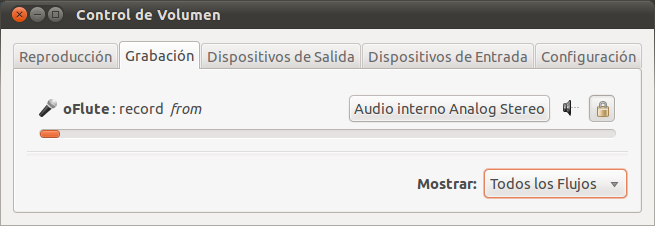
\includegraphics[width=0.7\textwidth]{6_implementacion/imagen_pavucontrol}
    \caption{Control de volumen, mostrando el cliente \textit{oFlute}}
  \end{figure}
\item[Tipo de flujo] En nuestro caso será de entrada, por lo que se utilizó la
  macro \texttt{\nohyphens{kPA\_STREAM\_RECORD}}.
\item[Tipo de \textit{sample}] Definirá el tipo de datos que se usará para
  representar los sonidos.
\item[Opciones de búffering] Según busquemos rendimiento, fiabilidad, poca
  latencia... tendremos que variar las opciones de búffering.
\end{description}

Una vez hayamos creado un flujo, que correrá en segundo plano, tendremos que
leer los datos que arroja. Para ello, la API simple de PulseAudio provee la
función \texttt{pa\_simple\_read}, que nos permitirá volcar en un búffer
temporal un fragmento de audio. La elección del \textbf{tamaño del búffer} es
otro de los valores que repercutirá enormemente en el rendimiento del sistema.

Finalmente, una vez hayamos terminado de leer datos, podremos liberar el flujo
utilizando \texttt{pa\_simple\_free}. Con esto, ya podremos abrir, leer y cerrar
el flujo de sonido del micrófono. 

La parte más compleja a la hora de tratar con flujos es la de elegir los
parámetros apropiados. Son muchísimos los valores que hay que configurar:
frecuencia de muestreo, tamaño del búffer, número de canales, longitud del
búffer intermedio, latencia deseada\ldots Si no sabemos exactamente en qué
influye cada uno, acabamos en un proceso de prueba y error que puede resultar
muy tedioso.

\subsection{Análisis del audio capturado}

La segunda parte del proceso consiste en procesar y analizar el audio capturado
en cada momento, de forma que podamos conocer qué nota se está tocando con la
flauta a través del micrófono.

Como se ha comentado previamente, el alma del procesamiento en este caso es la
aplicación de la \textbf{transformada rápida de Fourier}
(\ref{sec:fourier}). Esta herramienta será capaz de descomponer los fragmentos
de sonido en sus componentes de frecuencia. La biblioteca usada en este caso es
KissFFT~\cite{kissfft}, que da unos resultados muy buenos en cuanto a
rendimiento y precisión. 

En el caso que nos concierne, un procesamiento básico de la señal será
suficiente para poder discernir la nota, por lo que podremos trabajar con
transformadas de fourier reales (no complejas). Para ello, KissFFT ofrece
variantes de sus funciones, muy optimizadas.

El primer paso es inicializar la biblioteca. KissFFT es capaz de utilizar el
mismo búffer entre distintas iteraciones de un cálculo, por lo que ahorramos el
tiempo de guardar y liberar memoria. Esta inicialización se guarda en un objeto
de configuración.

\begin{minted}{cpp}
  kiss_fftr_cfg configFFT = kiss_fftr_alloc (BUFSIZE, 0, NULL, NULL);
\end{minted}

El siguiente paso será realizar el cálculo sobre el búffer de sonido.  La forma
en que el algoritmo FFT almacena sus resultados depende de dos parámetros
principalmente: la frecuencia de muestreo y el tamaño del búffer de entrada. En
el caso de la FFT real, KissFFT devuelve el espectro positivo, que contendrá
tantos valores (en forma de números complejos) como el búffer de entrada más
uno. Cada uno de estos elementos representará la intensidad (y fase) de una
componente de frecuencia en la muestra inicial.

Pero, ¿cómo asociamos cada componente a la frecuencia apropiada? Ahí es donde
entra la frecuencia de muestreo. En el vector que arroja el cálculo del FFT,
haremos una simple regla de tres: el primer elemento corresponderá a la menor
frecuencia (0Hz), y el mayor elemento a la mayor frecuencia audible (en nuestro
caso será 22050Hz, ya que la frecuencia de muestreo es de 44.1kHz, por el
teorema de Nyquist -- sección~\ref{sec:nyquist}).
$$
   \begin{array}{ccc}
       \textrm{Pos. final}  & \longrightarrow & 22050Hz\\
       \textrm{Pos. X} & \longrightarrow & \textrm{Frecuencia Y}
   \end{array}
$$

Una vez identificadas las frecuencias en el resultado de la operación, es
necesario computar la \textbf{magnitud} de cada una de ellas, hallando el módulo
del número complejo. Tras esto, la \textbf{frecuencia fundamental} (que
representará la nota que está tocando la flauta) \textit{debería} ser la que
mayor magnitud tenga.

\subsection{Acotando el resultado}
El siguiente paso fue analizar las frecuencias que proveía la flauta dulce para
las nueve notas que puede emitir utilizando técnicas básicas -- esto es, sin
contar las notas que se pueden emitir utilizando técnicas avanzadas, como tapar
a medias ciertos orificios. De este estudio se extrajeron los siguientes
resultados (tabla \ref{tab:frecuencias}).

\begin{table}[ht!]
  \centering
  \begin{tabular}[h]{|c|c|}
    \hline
    \textbf{Frecuencia aproximada} & \textbf{Nota} \\ \hline
    523.25 Hz & Do, octava 5\\ \hline
    592.163 Hz & Re, octava 5\\ \hline
    656.763 Hz & Mi, octava 5\\ \hline
    699.829 Hz & Fa, octava 5\\ \hline
    785.692 Hz & Sol, octava 5\\ \hline
    893.628 Hz & La, octava 5\\ \hline
    1001.29 Hz & Si, octava 5\\ \hline
    1076.66 Hz & Do, octava 6 \\ \hline
    1195.09 Hz & Re, octava 6 \\ \hline
  \end{tabular}
  \caption{Frecuencias aproximadas de las notas de la flauta dulce}
  \label{tab:frecuencias}
\end{table}

Redondeamos el rango de frecuencias a $[450, 1500]$, cualquier sonido fuera de
ese rango no se considera una nota válida. En el resto de casos, se compara la
frecuencia fundamental obtenida con los valores en la tabla, y se devuelve la
nota apropiada.

\subsection{Ejecución concurrente}

Uno de los problemas que se encontraron fue que, inicialmente, el proceso de
análisis se incluyó dentro de la fase de cálculo de la lógica dentro del
\textit{game loop}. El resultado fue bastante poco satisfactorio, ya que el
cálculo de la FFT ralentizaba mucho el hilo, que tenía que esperar a que
concluyera para seguir renderizando el siguiente fotograma.

Así, se decidió, como suele ser habitual en el desarrollo de videojuegos, mover
el control y análisis del audio a un hilo aparte. Para ello, se hizo uso de la
biblioteca de hilos de Boost, que resulta mucho más amigable y sencilla de usar
que otras alternativas como los \textit{POSIX Threads}. 

A nivel de implementación, el uso de hilos en Boost es muy sencillo. Es
necesario tener una clase con el operador de función -- esto es,
\texttt{operator()} -- sobrecargado. Creamos un objeto de esa clase y se lo
pasamos al constructor de \texttt{boost::thread}, que llamará al anteriormente
citado operador en una copia del objeto pasado.

\begin{minted}{cpp}
// Instancia de la clase
ClaseCallable objeto;

// Hilo, crea una copia de objeto y llama al operador ()
boost::thread hilo(objeto);

// [...]

// Esperamos a que termine el hilo
hilo.join();
\end{minted}

Uno de los problemas que rápidamente se encontraron fue que, al lanzar el hilo,
se hace una copia del objeto referenciado. Esto resultaba un problema, ya que el
analizador hace cierta inicialización previa, y al duplicarse el objeto ocurrían
problemas. El resultado fue utilizar \texttt{boost::ref}, que permite pasar
referencias por copia.

\begin{minted}{cpp}
// Hilo sobre el propio objeto, no se hace copia
boost::thread hilo(boost::ref(objeto));
\end{minted}

\section{Gestión de estados}
\label{sec:implementacion_estados}

La gestión de estados es uno de los retos principales a la hora de desarrollar
un videojuego. Es necesario contar un sistema de gestión de estados robusto, que
permita pasar de un estado a otro de forma sencilla, sin errores, y manteniendo
información entre transiciones si fuera necesario.

En el caso de \textbf{oFlute}, el gestor de estados no necesitaba funciones
avanzadas; las secciones son consecutivas, por lo que no hay necesidad de
incluir concurrencia. Así pues, se editó el gestor de estados en base a la clase
\texttt{Gosu::Window}. Esta clase modela, mediante métodos, las diferentes fases
del \textit{game loop}, a saber:
\begin{enumerate}
\item Gestión de la entrada del usuario, mediante los métodos
  \texttt{buttonDown} y \texttt{buttonUp}.
\item Procesamiento de la lógica, en el método \texttt{update}.
\item Dibujado de los gráficos, en el método \texttt{draw}.
\end{enumerate}

Así, se creó una clase \texttt{Estado} con los mismos métodos, y una clase
\texttt{Juego} (heredera de \texttt{Gosu::Window}), que sirviese de controlador
de estados. Inicialmente, el gestor tenía un método \texttt{cambiarEstado}, que
descargaba de memoria el estado actual y cargaba el siguiente. Durante un tiempo
funcionó bien, pero llegó un momento en que empezaron a aparecer fallos de
memoria difíciles de acotar.

Tras bastantes días de depuración, finalmente el problema se encontró en el
\textit{momento} en el que se hacía la carga y descarga de estados. El conflicto
surgía porque se hacían llamadas para cambiar de estado \textit{en cualquier
  momento}, ya fuera en la etapa de lógica, de dibujado, o de gestión de la
entrada. En el instante de la llamada, se descargaba el estado actual y se
cargaba el siguiente. Esto originaba que las tareas que se habían lanzado, como
por ejemplo las imágenes pendientes de dibujar, se ejecutasen sobre objetos que
habían sido reemplazados en memoria. A menudo las imágenes se encontraban en
búferes de Gosu y no había problema, pero una vez se integró el analizador de
notas, el sistema empezó a fallar.

\label{sec:resolucion_problema_estados}

La solución fue bastante trivial. Se creó un sistema con una pequeña cola de un
elemento en el gestor de estados (la clase \texttt{Juego}). En el momento en que
alguien quisiese cambiar de estado, se añadía a la cola el nuevo estado a
cargar, y se activaba una bandera. Tras completar esa iteración del \textit{game
  loop}, al principio de la siguiente se hacía la carga y descarga de estados.

Este sistema de gestión de estados se extendió para incluir estados concurrentes
(por ejemplo, para mostrar menús de pausa), y aunque no se incluyó en oFlute,
está previsto su integración en la próxima versión de Freegemas~\cite{freegemas}.

%%% Local Variables: 
%%% mode: latex
%%% TeX-master: "../memoria"
%%% End: 
